\documentclass[12pt,fleqn]{article}\usepackage{../../common}
\begin{document}
Kesit Seviyeleri (Level Sets) ile İmaj Gruplamak 

Eğim (Curvature)

Kesit seviyeleri tekniğinde bir eğri normal formda değil, dolaylı
(implicit) bir fonksiyon ile $F(x,y) = 0$ olarak gösterilir. Bu fonksiyonun
tam diferansiyelini alırsak,

$$ dF = F_x dx + F_y dy = 0  $$

$$ dy = \frac{-F_x}{F_y}dx  $$

$$ y' = \frac{dy}{dx} = \frac{-F_x}{F_y} = f'(x) = \frac{df}{dx} $$

Burada bir faraziye daha var, o da aslında ilk verilen formülde olmasa bile
$y=f(x)$ olarak kabul etmemiz, yani $F(x,y)$ nasıl bir formül olursa olsun,
$y$'nin $x$'leri içerecek şekilde tekrar düzenlenebileceğini farz etmemiz,
böylece $F(x,f(x))$ olabileceğini söylemiş oluyoruz.

Şimdi $y'$ ifadesinin türevini bir daha alalım. Yukarıdaki $y'$ formülünde
en sağ taraf bir bölme işlemi içerdiği için burada Calculus'un Bölümler
Kuralını (Quotient Rule) uygulamamız lazım (detaylar için Bölüm Kuralı
yazısına bakınız). Bu kural şöyle gösterilir:

$$ \frac{d}{dx}\bigg(\frac{u}{v}\bigg) = 
\frac{\displaystyle \frac{v du}{dx} - \frac{u dv}{dx}}{v^2} $$

Bölümler Kuralı için $u$ ve $v$ tanımları nedir? 

$$ u = -F_x(x,f(x))  $$

$$ v = F_y(x,f(x)) $$

O zaman

$$ 
v \frac{du}{dx} = F_y \frac{dF_x}{dx} 
\mlabel{1}
$$

$$
u \frac{dv}{dx} = -F_x \frac{dF_y }{dx} 
\mlabel{2}
$$

Bunlardan mesela $dF_x/dx$ üzerinde Zincirleme Kanunu (Chain Rule) uygulamak
lazım (bu kural tam integral kuralının bir sonucu). 

$$ \frac{d F_x(x,f(x)) }{dx} = \frac{\partial F_x}{\partial  x}(x,f(x))+\frac{\partial F_x}{\partial y}\frac{df}{dx}\\ $$

$$
= F_{xx}(x,f(x))+F_{xy}(x,f(x))f'(x) 
\mlabel{3}
$$

$$
\frac{d F_y(x,f(x)) }{dx} =  F_{xy}(x,f(x))+F_{yy}(x,f(x))f'(x) 
\mlabel{4}
$$

Zincirleme Kanunu niye üstteki şekilde açıldı? Tam Diferansiyeli bir daha
hatırlayalım:

$$ df = \frac{\partial f}{\partial x} dx + \frac{\partial f}{\partial y} dy  $$

$$ \frac{df}{dx} = \frac{\partial f}{\partial x} \frac{dx}{dx} + \frac{\partial f}{\partial y} \frac{dy}{dx}  $$

$$ \frac{df}{dx} = \frac{\partial f}{\partial x} + \frac{\partial f}{\partial y} \frac{dy}{dx}  $$

O zaman formüller (1) (2) (3) ve (4) bir araya konulursa,

$$ y '' = - \frac{F_yF_{xx} - F_y F_{xy}\frac{F_x}{F_y} - F_xF_{xy} + F_xF_{yy}\frac{F_x}{F_y}}{F_y^2}\\ $$

$$ y '' = - \frac{F_yF_{xx} - F_{xy}F_x - F_xF_{xy} + \frac{F_x^2F_{yy}}{F_y}}{F_y^2} $$

Üstteki bölümün hem bölen, hem bölünen terimlerini $F_y$ ile çarparsak, ve
sadeleştirirsek

$$ y '' = - \frac{F_y^2F_{xx} - 2F_{xy}F_xF_y + F_x^2F_{yy}}{F_y^3} $$

Şimdi surada [2] türetimi gösterilen eğim  formülüne
bakalım. Not: Eğer

$$ \kappa = \frac{x'y''-y'x''}{\bigg(x'^2 + y'^2 \bigg)^{3/2}} $$

formülünün alttaki formüle nasıl dönüştüğü tam anlaşılır değilse,
hatırlayalım ki, $y=f(x)$, ve $x'=1$, ve $x'' = 0$.

Bu formülün Courant [1] sf. 231'de benzer bir formunu görüyoruz (Bu arada o
karmaşık formül yerine yaklaşıksal olarak hesaplama sırasında sadece $f''$
kullanmak ta mümkün [3, giriş bölümü])

$$ \kappa = \frac{f''}{(1+f'^2)^{3/2}} $$

Bu formüldeki $f''$ yani $y''$ için üstte bulduğumuz sonucu, $f'$ yani $y'$
için bu yazının başındaki formülü koyarsak,

$$ 
\kappa = \frac
{-\frac
{\displaystyle F_y^2F_{xx} - 2F_{xy}F_xF_y +  F_x^2F_{yy}}{\displaystyle F_y^3}}
{(1+f'^2)^{3/2}} 
$$  

Bölen kısmı nedir?

$$ (1+f'^2)^{3/2} = \bigg( 1 + \bigg(\frac{-F_x}{F_y}\bigg)^2 \bigg)^{3/2}  $$

$$ = \bigg( 1 + \frac{F_x^2}{F_y^2} \bigg)^{3/2}  $$

$$ = \bigg( \frac{F_y^2 + F_x^2}{F_y^2} \bigg)^{3/2}  $$

$$ = (F_y^2 + F_x^2)^{3/2}(F_y^{-2})^{3/2}  $$

$$ = (F_y^2 + F_x^2)^{3/2}F_y^{-6/2}  $$

$$ = (F_y^2 + F_x^2)^{3/2}F_y^{-3} $$

Yerine koyarsak,

$$ 
\kappa = \frac{\displaystyle
- \frac{F_y^2F_{xx} - 2F_{xy}F_xF_y + F_x^2F_{yy}}{F_y^3}}
{(F_y^2 + F_x^2)^{3/2}F_y^{-3}}
 $$

$F_y^{-3}$ ve $F_y^{3}$ birbirlerini iptal ederler ve sonuç:

$$
\kappa = \frac{F_y^2F_{xx} - 2F_{xy}F_xF_y +
    F_x^2F_{yy}}{(F_y^2 + F_x^2)^{3/2}}
\mlabel{5}
$$

Üstteki ünlü eğim  formülüdür. 

Bu eğim formülünün diğer bir şekli şöyledir ($F$ yerine $\phi$ kullanırsak)

$$ \kappa = \bigtriangledown \cdot \frac{\bigtriangledown \phi}{|\bigtriangledown \phi|} $$

Bunun okunuş şekli ``birim normal gradyanın uzaklaşım ölçüsü (divergence of the
unit normal gradient)'' şeklindedir. Acaba bu formül, (5). formül ile
uyumlu mu?

$$ \kappa = \nabla \cdot \frac{\nabla \phi}{|\nabla \phi|}  $$

$$ = \nabla \cdot \frac{(\phi_x,\phi_y)}{\sqrt{\phi_x^2+\phi_y^2}} $$

$$ = \left(\partial_x \frac{\phi_x}{\sqrt{\phi_x^2+\phi_y^2}}\right)+ 
\left(\partial_y \frac{\phi_y}{\sqrt{\phi_x^2+\phi_y^2}}\right)  $$

$$ = \frac{\phi_{xx}}{\sqrt{\phi_x^2+\phi_y^2}} - \frac{\phi_x (\phi_x\phi_{xx}+\phi_y\phi_{xy})}
{(\phi_x^2+\phi_y^2)^{3/2}} +
\frac{\phi_{yy}}{\sqrt{\phi_x^2+\phi_y^2}} - \frac{\phi_y(\phi_x\phi_{xy}+\phi_y\phi_{yy})}
{(\phi_x^2+\phi_y^2)^{3/2}}  $$

$$ = \frac{\phi_{xx}(\phi_x^2+\phi_y^2) - \phi_x
  (\phi_x\phi_{xx}+\phi_y\phi_{xy}) +\phi_{yy}(\phi_x^2+\phi_y^2) -
  \phi_y(\phi_x\phi_{xy}+\phi_y\phi_{yy})}{(\phi_x^2+\phi_y^2)^{3/2}} $$

$$ = \frac{\phi_{xx}\phi_y^2 - 2\phi_x\phi_y\phi_{xy} + \phi_{yy}\phi_x^2}{(\phi_x^2+\phi_y^2)^{3/2}}  $$

Bu formül bizim (5). formül ile tıpatıp aynı.

Üstteki işlemlerde uzaklaşım ölçüsü (divergence) operatörü $\nabla \cdot$
ile gradyan operatörü $\nabla$ arasındaki farkı belirtelim: $\nabla \cdot$
operatörü $F(x,y)$ üzerinde kısmi türevlerin toplamını verir, yani bir
skalar tek sayı döndürür. Gradyan ise her bir elemanı bir kısmi türeve
tekabül eden bir {\em vektör} geri getirir.

Python Numpy kodlaması bağlamında, daha önce {\em Kesit Seviyeleri} yazısında
ayrıksal olarak bir \verb!phi! değişkeni içindeki bir fonksiyon üzerinde
eğimselliği şöyle hesaplamıştık:


\begin{minted}[fontsize=\footnotesize,linenos,xleftmargin=1cm]{python}
gradPhiY, gradPhiX = np.gradient(phi)
absGradPhi=np.sqrt(gradPhiX**2+gradPhiY**2)                               

normGradPhiX=gradPhiX/(absGradPhi+(absGradPhi==0))
normGradPhiY=gradPhiY/(absGradPhi+(absGradPhi==0))

divYnormGradPhiX, divXnormGradPhiX=np.gradient(normGradPhiX)
divYnormGradPhiY, divXnormGradPhiY=np.gradient(normGradPhiY)
                       
K = divXnormGradPhiX + divYnormGradPhiY
\end{minted}

Bu satırların $\nabla \cdot \frac{\nabla \phi}{|\nabla \phi|}$ ifadesiyle
birebir uyum gösterdiğini herhalde görebiliyoruz. Satır 1, $\nabla \phi$
ifadesidir. Satırlar 4-5 $\frac{\nabla \phi}{|\nabla \phi|}$ işlemini
gerçekleştiriyor, gradyanı onun uzunluğuna (magnitude) bölerek onu birim vektörü
haline getiriyor. Satırlar 7-10 tekrar sonucun gradyanını bir daha alıyor, ama
bu sefer hesapsal kısmi türevleri birbiriyle topluyor, böylece uzaklaşım ölçüsü
(divergence) hesaplanmış oluyor. Tüm bu işlemlerin sonucu eğimsellik $\kappa$
oluyor.

Dikkat edilirse Python kodundaki K yani $\kappa$, N x N boyutlu bir matristir,
bu mantıklı çünkü $\kappa$ hesabı için kullandığımız $F_x$, $F_y$ gibi
türevler aslında $F_x(x,y)$, $F_y(x,y)$ formüllerine sahipler, yani her $x,y$
kombinasyonu için farklı bir sonuç döndürebilirler. Bu sebeple K yani $\kappa$
$\phi$ fonksiyonunun her $x,y$ noktası için tanımlıdır. 

Bazen literatürde $\nabla \cdot$ yerine $div(..)$ kullanıldığını görebilirsiniz,
bu operatörlerin ikisi de aynıdır.

Kesit Seviyeleri, Kenar Bazlı İmaj Gruplamak

Bir dijital imajı renklere, objelere göre belli parçalara bölmek
(segmentation) için, matematiksel bir formül kullanmak iyi çözümlerden
biridir. Bunu yapmanın bazı yolları var. Basitleştirerek bir örnek
verelim: diyelim ki gruplama için elimizdeki formül bir yuvarlak
formülü $x^2+y^2 - c = 0$, ki $c$ bir sabit. Bu formülü x ve y
kordinatları üzerinde bastığımız zaman radius'u $\sqrt{c}$ olan bir
çember elde ederiz. Gruplama için bu çemberi büyütüp
küçültebildiğimizi farzedelim, çember imaj üzerindeki istediğimiz
bölüme en iyi uyduğu anda gruplamayı başarılı olarak kabul ediyoruz.

Fakat problem şurada: eğer imajda birden fazla grup var ise, o zaman
birden fazla çember gerekecektir, bu sefer algoritmik olarak üstteki
formülü ikinci, üçüncü kere yaratmamız, ve o formüllerin o gruplara
uyumunu ayrı ayrı takip etmemiz gerekirdi. Ya da diyelim ki özyineli
(iterative) bir uydurma işlemi takip ediyoruz, bu işlem sırasında
belki iki çemberin birleşmesi gerekse, o zaman iki formülü silip,
yerine yenisini oluşturmakla uğraşmak gerekli olacaktı. Bunlar hem
matematiksel, hem kodlama açısından külfet oluşturacaktır.

Kesit Seviyeleri kavramını kullanarak bu işi daha
basitleştirebiliriz. Diyelim ki bölme görevini yapan $\phi$ adli
fonksiyonumuzu 2 boyutlu olmak yerine 3 boyutlu eksende tanımladık,
ve, 2 boyutta bölme yapma görevini onun bir kesitine verdik. Kesit
derken, alttaki üç boyutlu fonksiyonu yatay olarak bir noktadan
``kestiğimizi'' farz ediyoruz, ve o kesit üzerinde düşen $\phi$
değerlerine bakıyoruz.

Bakıç açışımızı, tanımlamamızı değiştirerek, bazı avantajlar elde
etmeyi umuyoruz aslında. Altta iki tane $\phi$ fonksiyonu ve onların
altında kesitlerini görebiliriz.


Kesit Seviyeleri tekniğini kullanarak elde ettiğimiz avantaj nedir?
Artık sadece \textbf{tek} bir $\phi$ fonksiyonu kullanarak 2 boyutlu
imajımız üzerinde birbirinden ayrı gruplamalar yaratabiliyoruz. Bu
gruplar birbiri ile birleşebilir, ayrılabilir, bu artık bizi
ilgilendirmiyor. Biz sadece 3. boyuttaki $\phi$ fonksiyonunu
değiştirmekle uğraşacağız, imaj üzerindeki gruplamalar ise o
fonksiyonun 2. boyuta yansıması (projection) üzerinden kendiliğinden
gerçekleşecekler.

Matematiksel olarak $\phi$ fonksiyonunu nasıl temsil ederiz? $\phi$
fonksiyonu $x$, $y$, boyutlarını alıp bize bir üçüncü $z$ boyutu
döndürmeli, ayrıca bu fonksiyonu imajı parçalarına ayırma işlemini
gerçekleştirmek için kademeli olarak değiştirmeyi planladığımıza göre,
o zaman bir $t$ değişkeni de gerekiyor. Yani $\phi(x,y,t)$
fonksiyonu. Gruplama için kullanılacak kesiti ise sıfır kesiti olarak
alalım, yani $\phi(x,y,t) = 0$. Doğal olarak

$$ \frac{d}{dt}(\phi(x,y,t) = 0) = 0 $$

Şimdi $x$, ve $y$ değişkenlerinin zaman göre değişimini formüle bir
şekilde dahil etmek lazım. Bunun için sıfır kesit seviyesi üzerinde
bir parçacık hayal edilir, ve bu parçacığın gittiği yol $x(t)$, ve
$y(t)$ olarak tanımlanır. O zaman

$$ \frac{d}{dt}(\phi(x(t),y(t),t)) = 0 $$

Tam diferansiyel formülünden hareketle:

$$ 
d(\phi(x(t),y(t),t) = 
\frac{\partial \phi}{\partial x}dx + 
\frac{\partial \phi}{\partial y}dy + 
\frac{\partial \phi}{\partial t}dt  = 0
 $$

$$ 
\frac{d(\phi(x(t),y(t),t))}{dt} = 
\frac{\partial \phi}{\partial x}\frac{dx}{dt} + 
\frac{\partial \phi}{\partial y}\frac{dy}{dt} + 
\frac{\partial \phi}{\partial t} = 0
 $$

$$
 = 
\frac{\partial \phi}{\partial x}\frac{dx}{dt} + 
\frac{\partial \phi}{\partial y}\frac{dy}{dt} + 
\phi_t = 0
\mlabel{1}
$$

Temsilen daha kısa bir işaret kullanmak gerekirse, $\bigtriangledown$
ile $\phi$'nin gradyanını (gradient) alarak, elde edilecek vektörün
nokta çarpımını kullanabiliriz.  O zaman formül (1) daha kısa
olarak:

$$ \phi_t + \bigtriangledown \phi \cdot \vec{V} = 0 $$

olarak temsil edilebilir, ki

$$ \bigtriangledown \phi = \bigg(
\frac{\partial \phi}{\partial x},
\frac{\partial \phi}{\partial y} \bigg)
 $$

$$ \vec{V} = \bigg(
\frac{dx}{dt} ,
\frac{dy}{dt} \bigg)
 $$

İki vektörün nokta çarpımı bilindiği gibi sırayla her iki vektörün
sırasıyla uyan elemanlarının birbirleri ile çarpılması ve o
çarpımların toplanmasıdır.

$\vec{V}$ vektörü neyi temsil eder? Formüle göre bu vektör $\phi$'nin
üzerindeki değişimi etkiliyor, ve bu değişimler $t$'nin değişimine
göre tanımlandığına göre bu değerler ``hız'' olarak
tanımlanabilir. İmaj bağlamında düşünürsek mesela $\phi$ renklerin
aynı olduğu yerlerde yüksek hızda, renklerin değiştiği yerler düşük
hızda değişebilir şeklinde bir kurgu yapılabilir, işte bu bölgelerde
değişiminin hızını $\vec{V}$ ile gösterebiliriz.

$\vec{V}$ yerine kesit seviyelerine dik olan (normal) vektörler ile çalışmak
isteseydik, $\vec{V}$'yi dik ve teğet bileşenlerine ayırarak tekrar temsil
edebilirdik: $\vec{V} = V_N\vec{N} + V_T\vec{T}$. Bu formülde $\vec{T}$ teğet,
$\vec{N}$ dik vektörler, $V_N$ ve $V_T$ skalar. Yerine koyalım:

$$ \phi_t + \bigtriangledown \phi \cdot (V_N\vec{N} + V_T\vec{T}) = 0 $$

$\phi$'ye göre dik vektörün diğer bir formülü $\vec{N} =
\frac{\bigtriangledown\phi}{|\bigtriangledown\phi|}$ olduğuna göre

$$ \phi_t + (\bigtriangledown \phi \cdot
V_N\frac{\bigtriangledown\phi}{|\bigtriangledown\phi|} + \bigtriangledown
\phi \cdot V_T\vec{T}) = 0 $$

Devam edelim: $\bigtriangledown \phi$ yüzeye dik olduğuna göre, bu dik vektörün
teğet olan $\vec{T}$ ile noktasal çarpımı sıfır değerini verecektir, o çarpım
formülden atılabilir. Kalanlar:

$$ \phi_t + (\bigtriangledown \phi \cdot 
V_N\frac{\bigtriangledown\phi}{|\bigtriangledown\phi|}) = 0 $$

Daha da kısaltabiliriz: $\bigtriangledown \phi \cdot \bigtriangledown \phi
= |\bigtriangledown \phi|^2$ olduğunu biliyoruz, gradyanın kendisi ile
noktasal çarpımı, o gradyan vektörünün uzunluğunun karesidir. Daha genel
olarak, bir vektörün uzunluğu, o vektörün kendisi ile noktasal çarpımının
kareköküdür. O zaman en son formülde bu çarpımı gerçekleştirip, uzunluk
olarak yazalım:

$$ \phi_t + V_N\frac{|\bigtriangledown\phi|^2}{|\bigtriangledown\phi|} = 0  $$

$$ \phi_t + V_N |\bigtriangledown\phi| = 0  $$

Şimdi bu formül hakkında biraz anlayış geliştirelim. Eğer elimizdeki
bir $\phi$ seviye kesitinin şeklen olduğu gibi kalmasını ama sadece
küçülmesini isteseydik, $\phi$'nin normalinin tersi yönünde bir büyüme
tanımlamamız gerekirdi. Normal vektör dışa doğru işaret ettiğine göre
üstteki formülde mesela $V_N = -1$ tanımlayabilirdik. O zaman

$$ \phi_t + -1 |\bigtriangledown\phi| = 0 $$

$$ \phi_t = |\bigtriangledown\phi|   $$

Hesapsal olarak bunu nasıl gerçekleştiririz? 80 x 80 boyutunda bir
matris içinde $\phi$ fonksiyonu ayrıksal olarak tutalım. Yani 80 tane
x, 80 tane ayrı y değeri var, her x ve y değerlerin kombinasyonlarına
tekabül eden $\phi$ değerleri bu matris içinde. Gradyanın ne olduğunu
hatırlayalım. Gradyan

$$ 
\bigtriangledown \phi = \bigg(
\frac{\partial \phi}{\partial x},
\frac{\partial \phi}{\partial y} \bigg)
$$

olarak tanımlıdır, ve her $(x_i,y_i)$ noktasındaki $\phi(x_i,y_i)$
değerine göre değişik bir vektör sonucunu getirecektir. Bilgisayar
dünyasında parçalı türevler hesapsal ``farklılıklara'' dönüşürler,
\verb!phi! matrisindeki farklılıkları Python ile

\begin{minted}[fontsize=\footnotesize]{python}
gradPhiY, gradPhiX = np.gradient(phi)
\end{minted}

olarak hesaplayabiliriz. Üstte elimize geçen gradyan dizinlerindeki
değerler ile $|\bigtriangledown\phi|$ büyüklüğünü hesaplayabiliriz, ve bu
sonucu $\phi$ üzerindeki değişim oranı $\phi_t$ olarak kabul ederiz. O
zaman $\phi_t$ ile zaman $t$ değimi \verb!dt! çarptığımız zaman ele geçecek
olan $\phi$'nin değişimidir. Döngünün her basamağında eski \verb!phi!
değerlerine bu farkları eklediğimiz zaman $\phi$ fonksiyonu istediğimiz
gibi evrilecektir.

Alttaki kodda bizim başlangıç $\phi$'miz kenarlardan w uzaklığında içi boş
bir kutu olacak. 

Ortalama Eğim (Mean Curvature) Kullanmak

Eğer sabit hız yerine sıfır kesit seviyesinin herhangi bir noktada ne kadar
``eğri'' olduğuna göre ilerlemesini işletseydik ne olurdu?  Diyelim ki çok
eğri bölgelerde çok hızlı, az eğik (düz, düze yakın) bölgelerde ilerleme az
hız istiyoruz. O zaman hangi şekille başlarsa başlasındalar $\phi$ kesiti
sonuçta bir çember şekline doğru evrilecektir. Ortalama eğim (mean
curvature) hesabı için şu denklem kullanılır:

$$ \kappa = -div \bigg( \frac{\bigtriangledown \phi}
{|\bigtriangledown \phi| } \bigg) $$

\begin{minted}[fontsize=\footnotesize]{python}
from mpl_toolkits.mplot3d import Axes3D
import numpy as np

def plot_phi(phi):
    fig = plt.figure()
    ax = Axes3D(fig)
    x = []
    y = []
    for (i,j),val in np.ndenumerate(phi):
        x.append(i)
        y.append(j)
    ax.plot(xs=x, ys=y, zs=phi.flatten(), 
            zdir='z', label='ys=0, zdir=z')

f, ax = plt.subplots()

# initial function phi - level set is a square 4 pixels
# away from borders on each side, in 3D it looks like an empty
# box
c0=2; w=2
nrow, ncol= (30,30)
phi=c0*np.ones((nrow,ncol))
phi[w+1:-w-1, w+1:-w-1]=-c0

dt=1.

phiOld=np.zeros((nrow,ncol))

iter=0

while iter < 50:
    # gradient of phi
    gradPhiY, gradPhiX = np.gradient(phi)
    # magnitude of gradient of phi
    absGradPhi=np.sqrt(gradPhiX**2+gradPhiY**2)                               
    
    # normalized gradient of phi - eliminating singularities
    normGradPhiX=gradPhiX/(absGradPhi+(absGradPhi==0))
    normGradPhiY=gradPhiY/(absGradPhi+(absGradPhi==0))
    
    divYnormGradPhiX, divXnormGradPhiX=np.gradient(normGradPhiX)
    divYnormGradPhiY, divXnormGradPhiY=np.gradient(normGradPhiY)
                           
    # curvature is the divergence of normalized gradient of phi
    K = divXnormGradPhiX + divYnormGradPhiY
    dPhiBydT = K * absGradPhi # makes everything circle
    
    # level set evolution equation    
    phi = phi + ( dt * dPhiBydT )
    if iter % 10 == 0: 
        CS = plt.contour(phi,0,colors='r')
        plt.hold(False)
        plt.savefig('level_1_'+ str(iter) + '.png')
        #plot_phi(phi)
        plt.savefig('phi_1_'+ str(iter) + '.png')
    iter += 1
\end{minted}

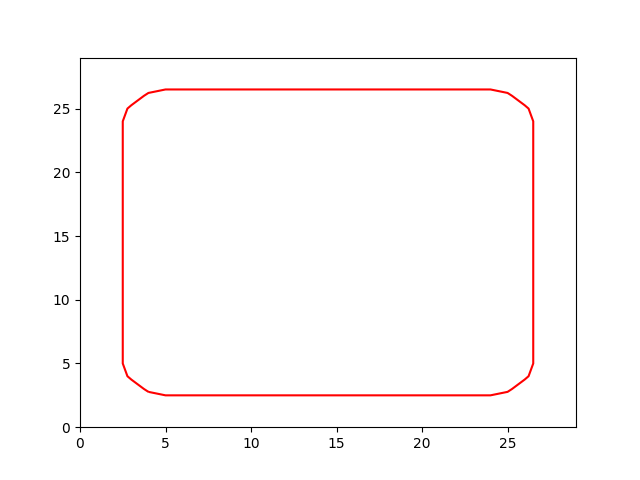
\includegraphics[height=4cm]{level_1_0.png}
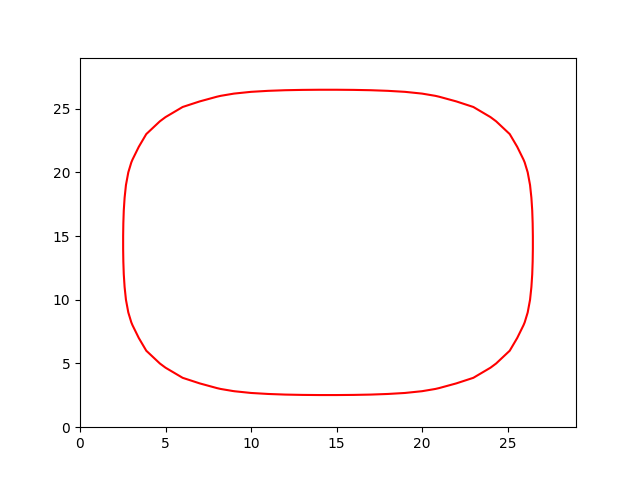
\includegraphics[height=4cm]{level_1_10.png}
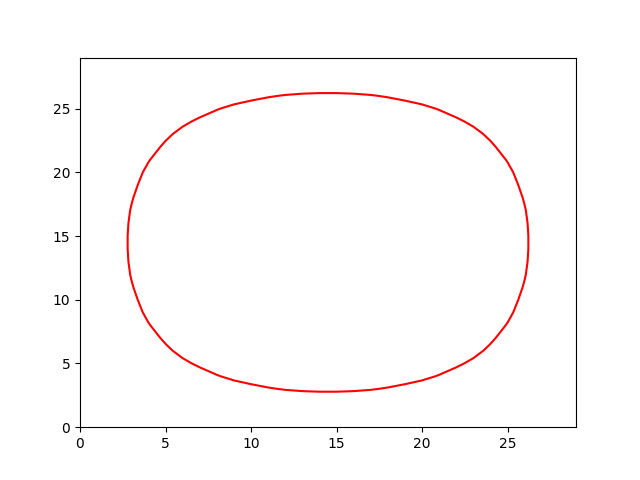
\includegraphics[height=4cm]{level_1_20.png}
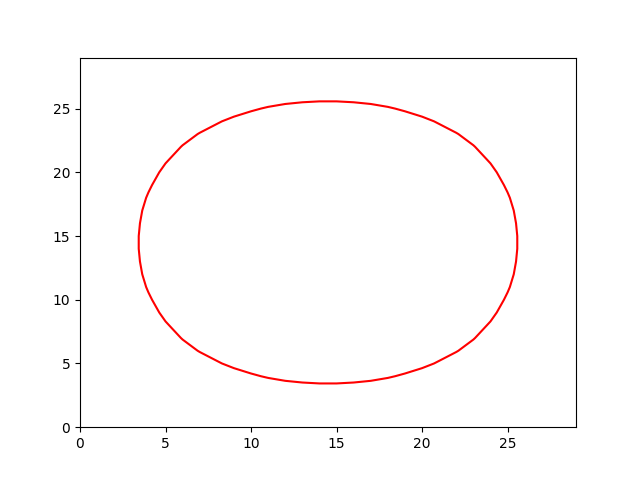
\includegraphics[height=4cm]{level_1_30.png}
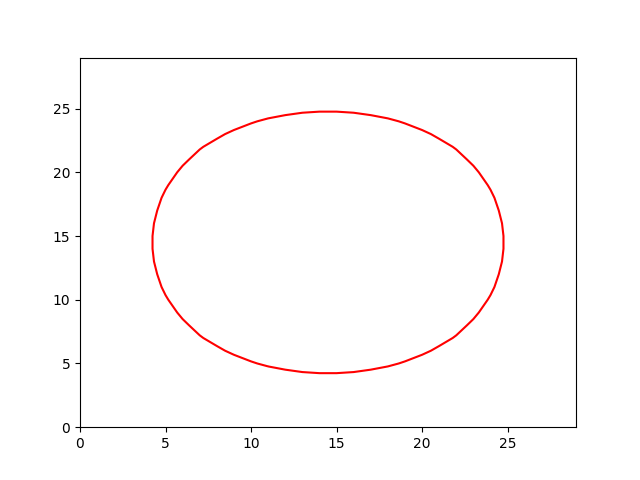
\includegraphics[height=4cm]{level_1_40.png}

İmaj Gruplamak

İmajı bölümlere ayırmak için (segmentation) birkaç faktörün bileşimi
kullanılıyor. Köşeleri kullanan aktif kontur (edge based active contour)
yönteminde ortalama eğim ve imajın piksel değerlerinin farklılıkları (image
gradient) aynı anda kullanılır. Yani kesit seviyesini ilerletirken hızı hem
eğime oranlıyoruz, hem de imaj piksel renk değerleri arasındaki farka ters
oranda hızlandırıyor, ya da yavaşlatıyoruz. Böylece kesit seviyemiz renk
farklılığı çok olmayan yani büyük bir ihtimalle tek bir objeye ait bir
bölgede hızla ilerliyor, büyük renk farkının olduğu büyük bir ihtimalle bir
kenar noktasına gelince ise yavaşlıyor. O sırada kesit seviyesinin geri
kalan tarafları tabii ki başka hızlarda hareket ediyor olabilirler, zaten
işin püf noktası burada, sonunda resim bölgelere ayrılmış oluyor.

Bitirirken önemli gözlemi vurgulayalım. Problemi matematiksel olarak temsil
ederken, hedefe doğru türetirken sürekli (continous) alemde, sürekli,
kesintisiz fonksiyonlarla iş yapıyoruz. Hesaplama anı gelince sürekli
fonksiyonları ayrıksal (discrete) hale çeviriyoruz, işte uygulamalı
matematiğin hesapsal kısmı burada devreye giriyor. Fakat diferansiyel
denklemler, fonksiyonlar, türevler gibi sürekli matematiğin kavramları çok
önemli, bunlar olmasa problemi soyut bir şekilde temsil edemez, ve
basitleştiremezdik. Temel matematiğin kavramlarını kullanırken yüzyılların
matematiksel bilgisi devreye girebiliyor, matematiğin en yoğun şekilde
kullanıldığı fizikten bol bol teknik alınabilir. Yani söylemek istediğimiz
problemi çözmek için hemen kodlamaya başlamıyoruz, düşünsel eylemin önemli
bir kısmı matematiksel formüllerle (belki kalem kağıtla) yapılıyor.

\begin{minted}[fontsize=\footnotesize]{python}
import scipy.signal as signal
import scipy.ndimage as image
import time

def gauss_kern():
    """ Returns a normalized 2D gauss kernel array for convolutions """
    h1 = 8
    h2 = 8
    x, y = np.mgrid[0:h2, 0:h1]
    x = x-h2/2
    y = y-h1/2
    sigma = 10.0
    g = np.exp( -( x**2 + y**2 ) / (2*sigma**2) );
    return g / g.sum()

Img = plt.imread("twoObj.bmp")
Img = Img[::-1] 
g = gauss_kern()
Img_smooth = signal.convolve(Img,g,mode='same')
Iy,Ix=np.gradient(Img_smooth)
absGradI=np.sqrt(Ix**2+Iy**2);
rows, cols = Img.shape

# initial function phi - level set is a square 4 pixels
# away from borders on each side, in 3D it looks like an empty
# box
c0=4
w=4
nrow, ncol=Img.shape
phi=c0*np.ones((nrow,ncol))
phi[w+1:-w-1, w+1:-w-1]=-c0

# edge-stopping function
g = 1 / (1+absGradI**2)

# gradient of edge-stopping function
gy,gx = np.gradient(g)

# gradient descent step size
dt=1

# number of iterations after which we reinitialize the surface
num_reinit=10

phiOld=np.zeros((rows,cols))

# number of iterations after which we reinitialize the surface
iter=0

while iter<150:
    # gradient of phi
    gradPhiY, gradPhiX = np.gradient(phi)    
    # magnitude of gradient of phi
    absGradPhi=np.sqrt(gradPhiX**2+gradPhiY**2)
    # normalized gradient of phi - eliminating singularities
    normGradPhiX=gradPhiX/(absGradPhi+(absGradPhi==0))
    normGradPhiY=gradPhiY/(absGradPhi+(absGradPhi==0))
    
    divYnormGradPhiX, divXnormGradPhiX=np.gradient(normGradPhiX)
    divYnormGradPhiY, divXnormGradPhiY=np.gradient(normGradPhiY)
                           
    # curvature is the divergence of normalized gradient of phi
    K = divXnormGradPhiX + divYnormGradPhiY
    tmp1 = g * K * absGradPhi
    tmp2 = g * absGradPhi
    tmp3 = gx * gradPhiX + gy*gradPhiY
    dPhiBydT =tmp1 + tmp2 + tmp3    
    
    phiOld=phi
    # level set evolution equation    
    phi = phi + ( dt * dPhiBydT )
    iter=iter+1
    if np.mod(iter,20)==0:
        f=plt.figure()
        plt.imshow(Img, cmap='gray')
        CS = plt.contour(phi,0, colors='r') 
        plt.savefig('level_2_' + str(iter) + '.png')
\end{minted}

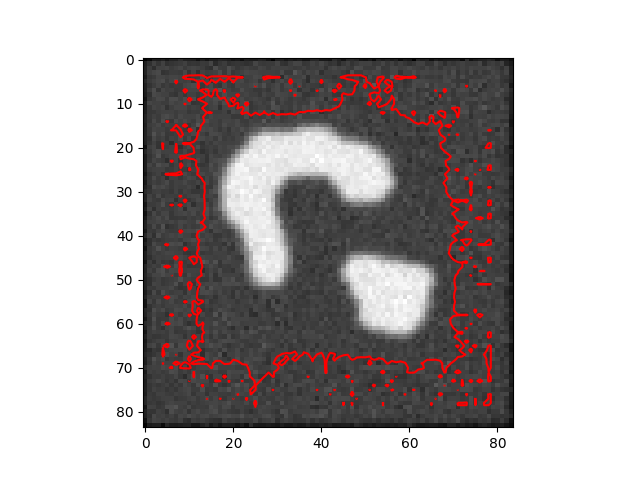
\includegraphics[height=4cm]{level_2_20.png}
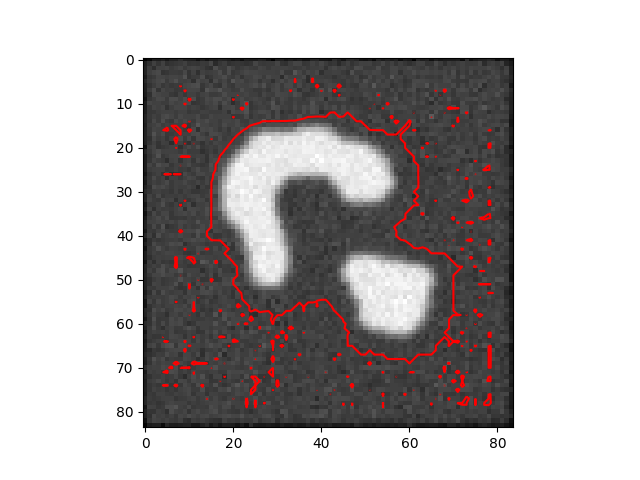
\includegraphics[height=4cm]{level_2_40.png}
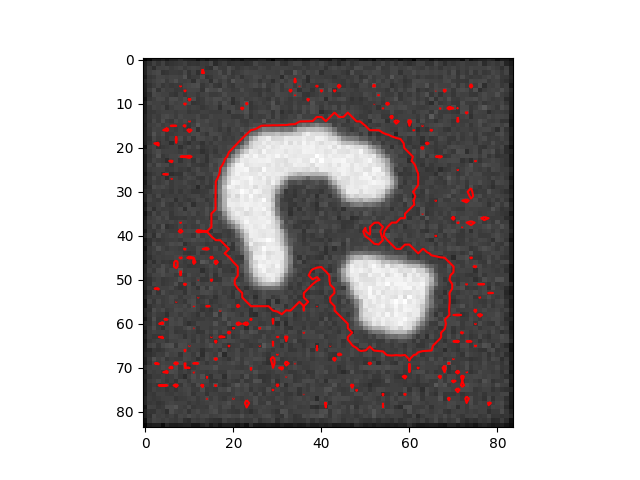
\includegraphics[height=4cm]{level_2_60.png}
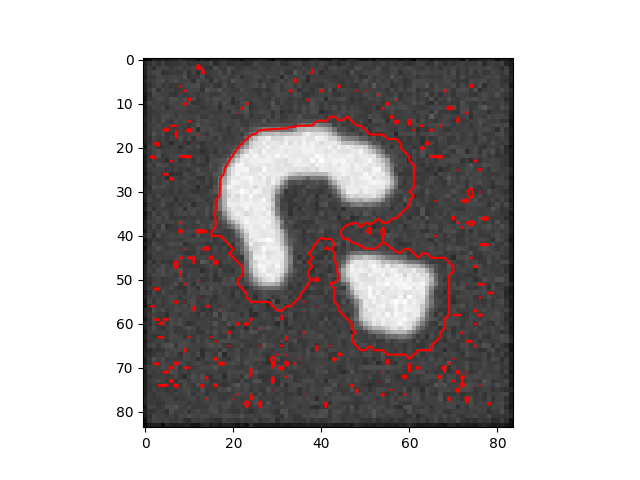
\includegraphics[height=4cm]{level_2_80.png}
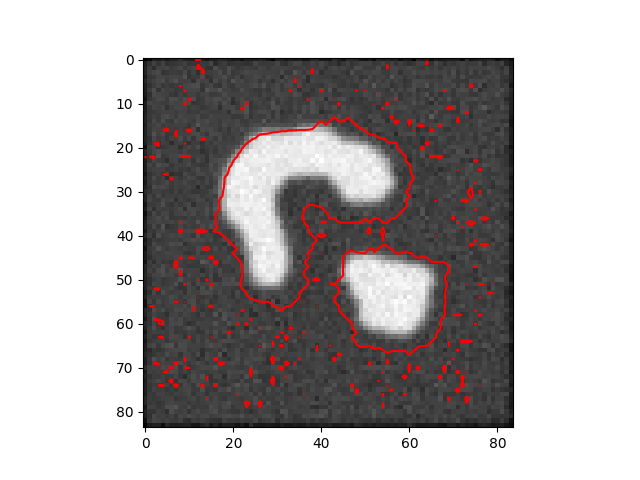
\includegraphics[height=4cm]{level_2_100.png}
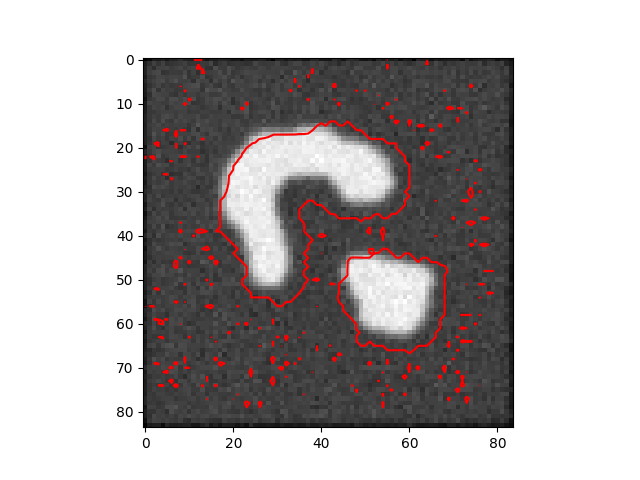
\includegraphics[height=4cm]{level_2_120.png}
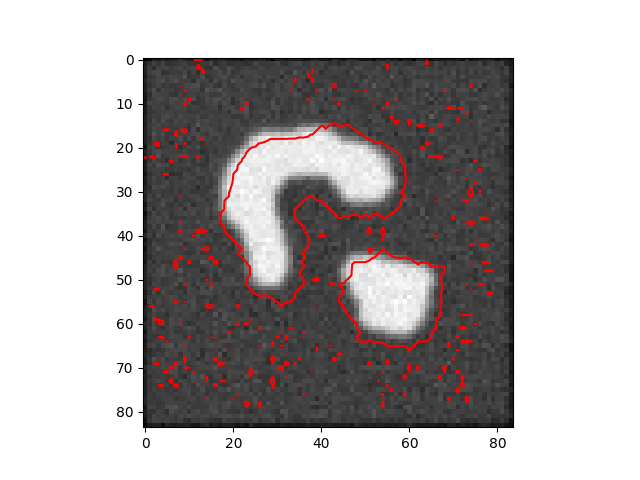
\includegraphics[height=4cm]{level_2_140.png}



Kaynaklar

[1] Courant, {\em Introduction to Calculus and Analysis Volume 2}, sf. 223-232

[2] Wolfram Mathworld, {\em Curvature}, \url{http://mathworld.wolfram.com/Curvature.html}

[3] Strang, {\em Computational Science and Engineering}, 

\end{document}

